% Guía completa del brazo XK-JS1-1 y de su gemelo digital (II-2026)
% Compilar desde esta carpeta:  pdflatex guia_completa_brazo.tex (dos o tres veces)
\documentclass[a4paper,11pt]{article}
% Estilo común de los manuales del gemelo digital (se incluye con \input)
\usepackage{geometry}
\geometry{letterpaper, margin=2.2cm}
\usepackage[spanish, es-nodecimaldot, mexico]{babel}
\usepackage[utf8]{inputenc}
\usepackage[T1]{fontenc}
\usepackage{lmodern}
\usepackage{amsmath,amssymb}
\usepackage[table]{xcolor}
\definecolor{naranja}{RGB}{194,98,12}
\definecolor{rojo}{RGB}{192,57,43}
\definecolor{verde}{RGB}{30,120,70}
\definecolor{azulw}{RGB}{0,103,184}
\definecolor{azulg}{RGB}{70,90,120}
\definecolor{gris}{RGB}{242,242,242}
\definecolor{grisos}{RGB}{90,90,90}
\usepackage{booktabs,longtable,array,tabularx}
\usepackage{graphicx}
\usepackage{float}
\usepackage{caption}
\captionsetup{font=small, labelfont=bf}
\usepackage{tikz}
\usetikzlibrary{positioning,arrows.meta,fit,calc,shapes.geometric,decorations.pathreplacing,backgrounds}
\usepackage{enumitem}
\setlist{itemsep=2pt}
\usepackage{listings}
\lstset{basicstyle=\ttfamily\small, frame=single, backgroundcolor=\color{gris}, breaklines=true,
  columns=fullflexible, keepspaces=true, extendedchars=true, upquote=true,
  literate={á}{{\'a}}1 {é}{{\'e}}1 {í}{{\'i}}1 {ó}{{\'o}}1 {ú}{{\'u}}1 {ñ}{{\~n}}1 {Á}{{\'A}}1 {É}{{\'E}}1
           {Í}{{\'I}}1 {Ó}{{\'O}}1 {Ú}{{\'U}}1 {Ñ}{{\~N}}1 {ü}{{\"u}}1 {¿}{{?`}}1 {¡}{{!`}}1 {…}{{...}}3
           {θ}{{$\theta$}}1 {·}{{$\cdot$}}1 {«}{{\guillemotleft}}1 {»}{{\guillemotright}}1 {°}{{$^\circ$}}1}
\usepackage{hyperref}
\hypersetup{colorlinks=true, linkcolor=naranja, urlcolor=naranja}
\usepackage{fancyhdr}
\pagestyle{fancy}
\fancyhf{}
\cfoot{\small \thepage}
\newcommand{\codigo}[1]{\texttt{#1}}
\newcommand{\archivo}[1]{\textbf{\texttt{#1}}}
\newcommand{\aviso}[1]{\par\smallskip\noindent\colorbox{rojo!10}{\parbox{\dimexpr\linewidth-2\fboxsep}{\textbf{\color{rojo}Atención.} #1}}\par\smallskip}
\newcommand{\nota}[1]{\par\smallskip\noindent\colorbox{gris}{\parbox{\dimexpr\linewidth-2\fboxsep}{#1}}\par\smallskip}
\tikzset{
  marca/.style={circle, fill=naranja, text=white, font=\bfseries\footnotesize, inner sep=1.4pt, minimum size=4.6mm, draw=white, line width=0.8pt},
  caja/.style={draw, rounded corners=2pt, fill=gris, align=center, font=\small, minimum height=10mm, inner sep=4pt},
  cajab/.style={caja, fill=white},
  cajan/.style={caja, fill=naranja!14, draw=naranja!70!black},
  paso/.style={draw, rounded corners=2pt, fill=white, align=left, font=\small, text width=3.4cm, minimum height=15mm, inner sep=5pt},
  num/.style={circle, fill=naranja, text=white, font=\bfseries\small, inner sep=1.5pt, minimum size=6mm},
  flecha/.style={-{Stealth[length=2.2mm]}, thick},
  dflecha/.style={{Stealth[length=2.2mm]}-{Stealth[length=2.2mm]}, thick},
  etiq/.style={font=\scriptsize, align=center},
}
\DeclareRobustCommand{\num}[1]{\tikz[baseline=-0.7ex]\node[marca]{#1};}
% \captura{ancho}{archivo}{marcas en coordenadas 0-1 desde la esquina inferior izquierda}
\newcommand{\captura}[3]{%
  \begin{tikzpicture}
  \node[anchor=south west, inner sep=0, draw=black!25] (img) {\includegraphics[width=#1]{#2}};
  \begin{scope}[x={(img.south east)}, y={(img.north west)}]
  #3
  \end{scope}
  \end{tikzpicture}}
% ventana dibujada (consolas y diálogos): \ventana{ancho}{alto}{título}{contenido}
\newcommand{\ventana}[4]{%
\begin{tikzpicture}
\node[draw=black!50, fill=white, minimum width=#1, minimum height=#2, anchor=north west, inner sep=0] (v) at (0,0) {};
\fill[black!8] (v.north west) rectangle ($(v.north east)+(0,-6mm)$);
\node[anchor=west, font=\scriptsize] at ($(v.north west)+(2mm,-3mm)$) {#3};
\node[anchor=east, font=\scriptsize] at ($(v.north east)+(-2mm,-3mm)$) {--\quad$\square$\quad$\times$};
\node[anchor=north west, inner sep=3mm, text width=#1-6mm, font=\scriptsize\ttfamily, align=left] at ($(v.north west)+(0,-6mm)$) {#4};
\end{tikzpicture}}

\lhead{\small Brazo XK-JS1-1 y su gemelo digital}
\rhead{\small Guía completa}
\lstdefinestyle{py}{language=Python, keywordstyle=\color{azulg}\bfseries, commentstyle=\color{grisos}\itshape,
  stringstyle=\color{verde}, basicstyle=\ttfamily\scriptsize, numbers=left, numberstyle=\tiny\color{grisos}}
\lstdefinestyle{js}{language=Java, morekeywords={const,let,function,async,await,return,for,of,if,else}, keywordstyle=\color{azulg}\bfseries,
  commentstyle=\color{grisos}\itshape, stringstyle=\color{verde}, basicstyle=\ttfamily\scriptsize, numbers=left, numberstyle=\tiny\color{grisos}}
\lstdefinestyle{awl}{basicstyle=\ttfamily\scriptsize, commentstyle=\color{grisos}\itshape, morecomment=[l]{//},
  keywordstyle=\color{azulg}\bfseries, morekeywords={LD,LDN,A,AN,O,ON,EU,ED,S,R,MOVB,MOVW,MOVD,PLS,TON,CALL,LPS,LRD,LPP,ALD,OLD}}

% -------------------------------------------------------------- símbolos ladder
\tikzset{
  ld/.style={line width=0.7pt},
  pics/na/.style={code={\fill[white](-0.12,-0.26) rectangle (0.12,0.26);
     \draw[thick](-0.1,-0.24)--(-0.1,0.24)(0.1,-0.24)--(0.1,0.24);
     \node[font=\scriptsize\ttfamily, above] at (0,0.22){#1};}},
  pics/nc/.style={code={\fill[white](-0.12,-0.26) rectangle (0.12,0.26);
     \draw[thick](-0.1,-0.24)--(-0.1,0.24)(0.1,-0.24)--(0.1,0.24);\draw(-0.17,-0.24)--(0.17,0.24);
     \node[font=\scriptsize\ttfamily, above] at (0,0.22){#1};}},
  pics/pf/.style={code={\fill[white](-0.12,-0.26) rectangle (0.12,0.26);
     \draw[thick](-0.1,-0.24)--(-0.1,0.24)(0.1,-0.24)--(0.1,0.24);
     \node[font=\tiny\bfseries] at (0,0){P};}},
  pics/cmp/.style n args={3}{code={\fill[white](-0.12,-0.26) rectangle (0.12,0.26);
     \draw[thick](-0.1,-0.24)--(-0.1,0.24)(0.1,-0.24)--(0.1,0.24);
     \node[font=\tiny\ttfamily] at (0,0){#2};
     \node[font=\scriptsize\ttfamily, above] at (0,0.22){#1};
     \node[font=\scriptsize\ttfamily, below] at (0,-0.22){#3};}},
  pics/bob/.style n args={3}{code={\fill[white](-0.2,-0.26) rectangle (0.2,0.26);
     \draw[thick](-0.05,0.24) arc (110:250:0.255);\draw[thick](0.05,0.24) arc (70:-70:0.255);
     \node[font=\tiny\bfseries] at (0,0){#2};
     \node[font=\scriptsize\ttfamily, above] at (0,0.22){#1};
     \node[font=\scriptsize\ttfamily, below] at (0,-0.22){#3};}},
  fb/.style={draw, fill=white, font=\scriptsize\ttfamily, align=left, inner sep=3pt, anchor=west},
  fbt/.style={font=\scriptsize\ttfamily\bfseries},
  barra/.style={line width=2pt},
  estado/.style={draw, rounded corners=3pt, fill=white, align=center, font=\scriptsize, minimum width=22mm, minimum height=10mm, inner sep=3pt},
  estadon/.style={estado, fill=naranja!14, draw=naranja!70!black},
  trans/.style={font=\scriptsize, align=center, fill=white, inner sep=1pt},
}

\title{\textbf{Brazo XK-JS1-1 y su gemelo digital}\\[4pt]\large Guía completa: planta, programas del PLC, modelado y software}
\author{ETN-902 / ETN-1034 / ETN-1000 · UMSA · II-2026}
\date{10 de noviembre de 2026}

\begin{document}
\maketitle
\thispagestyle{fancy}

\begin{abstract}
Esta guía describe por completo el brazo XK-JS1-1 del laboratorio y el gemelo digital construido sobre él: qué hace el brazo, cómo está formado, cómo se conectan sus partes, qué hacen los dos programas del PLC (explicados con diagramas ladder), cómo se modeló su cinemática, cómo se comunica la PC con el PLC y cómo está escrito el software (la app de Python y la página web). Los manuales de Linux y de Windows explican cómo instalar y usar la app; el documento de arquitectura profundiza en el protocolo PPI y en las páginas web. Los datos no medidos en la planta se marcan como \textbf{SUPUESTO}.
\end{abstract}

\tableofcontents
\newpage

% #####################################################################
\part{La planta}

\section{Qué hace el brazo}

El XK-JS1-1 es un brazo didáctico de \textbf{4 grados de libertad} que toma piezas pequeñas y las deja en otro lugar. Sus cuatro movimientos son:

\begin{center}\small
\begin{tabularx}{\linewidth}{>{\raggedright}p{2.6cm} >{\raggedright}X >{\raggedright\arraybackslash}p{4.6cm}}
\toprule
\textbf{Movimiento} & \textbf{Qué hace} & \textbf{Accionamiento}\\
\midrule
Base ($\theta$) & gira todo el brazo alrededor de un eje vertical & motor paso a paso + engranaje\\
Carro X ($s_X$) & desplaza el brazo hacia adelante o atrás: cambia el \emph{alcance} & motor paso a paso + husillo inferior\\
Carro Y ($s_Y$) & mueve un bloque que, por una biela, levanta o baja el brazo: cambia la \emph{altura} & motor paso a paso + husillo superior\\
Garra & abre o cierra las mordazas & salida Q0.7 del PLC (1 = cerrada)\\
\bottomrule
\end{tabularx}
\end{center}

\begin{figure}[H]
\centering
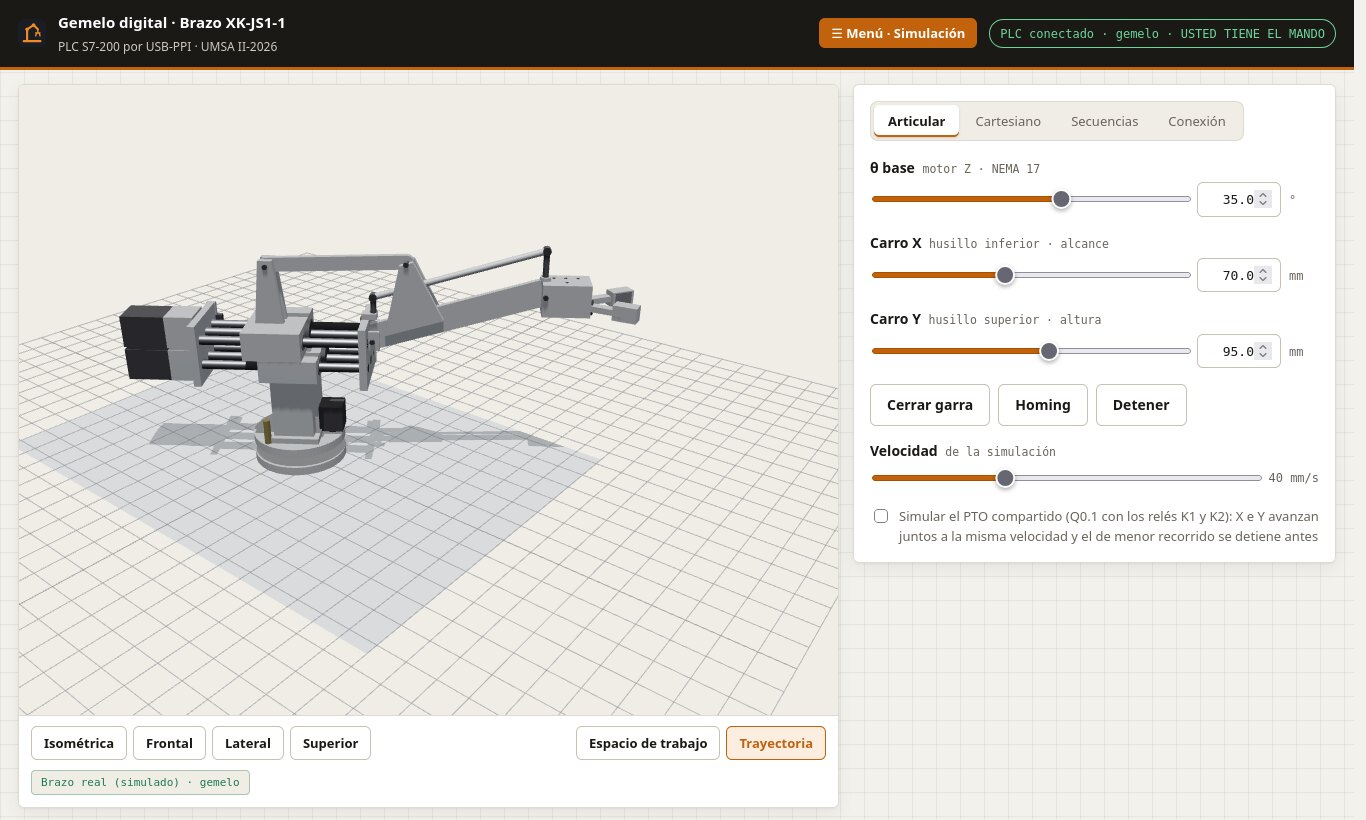
\includegraphics[width=0.78\linewidth, trim=0 60 520 50, clip]{img/local_articular.jpg}
\caption{El brazo dibujado por el gemelo digital con las mismas cotas que la máquina real ($\theta = 35^\circ$, $s_X = 70$~mm, $s_Y = 95$~mm).}
\end{figure}

En la planta original, el brazo solo podía moverse con los pulsadores del panel (modo manual) o repetir dos rutinas grabadas en el PLC (modo automático). Con el gemelo digital, además, se ve en 3D en tiempo real, se lleva a cualquier punto y se manda desde la PC o desde celulares.

% =====================================================================
\section{Componentes y cómo se conectan}

\begin{figure}[H]
\centering
\begin{tikzpicture}[node distance=7mm and 10mm]
\node[cajan, text width=3.1cm, minimum height=26mm] (plc) {\textbf{PLC S7-200}\\CPU 224 CN\\14 entradas\\10 salidas\\2 salidas de pulsos};
\node[caja, text width=2.6cm, above left=4mm and 14mm of plc] (panel) {panel:\\selector, paro,\\garra/inicio,\\6 pulsadores};
\node[caja, text width=2.6cm, below left=4mm and 14mm of plc] (sens) {finales de carrera X e Y\\sensor inductivo\\de la base};
\node[caja, text width=2.4cm, right=16mm of plc, yshift=16mm] (dz) {driver base\\JMC 2M542-N};
\node[caja, text width=2.4cm, right=16mm of plc, yshift=-4mm] (k) {relés K1 / K2\\reparten Q0.1};
\node[caja, text width=2.4cm, right=10mm of k, yshift=6mm] (dx) {driver X};
\node[caja, text width=2.4cm, right=10mm of k, yshift=-8mm] (dy) {driver Y};
\node[caja, text width=2.4cm, below=10mm of k] (garra) {garra};
\node[cajab, text width=1.6cm, right=6mm of dz] (mz) {motor\\base};
\node[cajab, text width=1.6cm, right=6mm of dx] (mx) {motor X};
\node[cajab, text width=1.6cm, right=6mm of dy] (my) {motor Y};
\node[cajab, text width=2.4cm, below=10mm of plc] (pc) {PC (cable USB-PPI,\\puerto 0)};
\draw[flecha] (panel) -- node[above, etiq, sloped]{I0.5--I1.5} (plc);
\draw[flecha] (sens) -- node[below, etiq, sloped]{I0.0--I0.4} (plc);
\draw[flecha] (plc.east) ++(0,0.6) -- node[above, etiq]{Q0.0, Q0.2} (dz.west);
\draw[flecha] (plc.east) ++(0,-0.4) -- node[above, etiq]{Q0.1} (k.west);
\draw[flecha] (k) -- node[above, etiq]{K1} (dx.west);
\draw[flecha] (k) -- node[below, etiq]{K2} (dy.west);
\draw[flecha] (plc.south east) -- node[above, etiq, sloped]{Q0.7} (garra.west);
\draw[flecha] (dz) -- (mz); \draw[flecha] (dx) -- (mx); \draw[flecha] (dy) -- (my);
\draw[dflecha] (plc) -- node[left, etiq]{PPI} (pc);
\node[etiq, above=1mm of dx] {DIR Q0.3};
\node[etiq, below=1mm of dy] {DIR Q0.4};
\end{tikzpicture}
\caption{Diagrama de bloques de la planta.}
\end{figure}

\subsection{Motores, drivers y transmisión}
Los tres ejes usan motores paso a paso NEMA 17 (200 pasos por vuelta) con drivers JMC 2M542-N. Cada driver recibe dos señales del PLC: \textbf{PUL} (un pulso = un micropaso) y \textbf{DIR} (sentido). La configuración de los interruptores DIP se leyó del tablero:

\begin{center}\small
\begin{tabular}{@{}llll@{}}
\toprule
\textbf{Interruptores} & \textbf{Posición} & \textbf{Significado} & \textbf{Efecto}\\
\midrule
SW1--SW3 & OFF OFF ON & corriente & 2,37~A pico\\
SW4 & OFF & corriente en reposo & la mitad al detenerse (menos calor)\\
SW5--SW8 & ON ON ON OFF & micropasos & 1000 pulsos por vuelta\\
\bottomrule
\end{tabular}
\end{center}

\begin{figure}[H]
\centering
\begin{tikzpicture}[node distance=4mm]
\node[cajan] (p) {1 pulso};
\node[caja, right=of p] (m) {$\frac{1}{1000}$ vuelta del motor};
\node[caja, right=of m] (h) {husillo de 5~mm/vuelta (SUPUESTO)};
\node[cajan, right=of h] (r) {0,005~mm de carro};
\draw[flecha] (p) -- (m); \draw[flecha] (m) -- (h); \draw[flecha] (h) -- (r);
\end{tikzpicture}
\caption{Cadena de transmisión de los carros X e Y: 200 pulsos por milímetro.}
\end{figure}

\begin{itemize}
\item \textbf{Carros X e Y}: $k = 1000 / 5 = 200$ pulsos/mm. Recorrido útil 0--170~mm (0--34\,000 pulsos) entre finales de carrera.
\item \textbf{Base}: la reducción no se conocía (el manual dice «engranaje»). Se calibró midiendo un giro con transportador: \textbf{190,3 pulsos por grado}. El sentido (Q0.2 = 0 positivo) es SUPUESTO.
\item \textbf{Velocidad}: a 4~kHz los carros avanzan $4000 / 200 = 20$~mm/s. Las salidas de pulsos llegan hasta 20~kHz, pero los programas no tienen rampas de aceleración, así que conviene no pasar de 4--5~kHz para no perder pasos.
\end{itemize}

\subsection{Mapa de entradas y salidas}
\begin{center}\small
\begin{tabularx}{\linewidth}{>{\ttfamily}p{1.1cm} >{\raggedright}X >{\ttfamily}p{1.1cm} >{\raggedright\arraybackslash}X}
\toprule
\textbf{\rmfamily Entrada} & \textbf{Función} & \textbf{\rmfamily Salida} & \textbf{Función}\\
\midrule
I0.0 & sensor inductivo de la base ($\theta = 0$) & Q0.0 & pulsos de la base (PTO0)\\
I0.1 & final de carrera X atrás (origen) & Q0.1 & pulsos de X e Y (PTO1), compartidos\\
I0.2 & final de carrera X adelante & Q0.2 & DIR base (1 = hacia el inductivo)\\
I0.3 & final de carrera Y abajo (origen) & Q0.3 & DIR X (0 = adelante, 1 = atrás)\\
I0.4 & final de carrera Y arriba & Q0.4 & DIR Y (0 = arriba, 1 = abajo)\\
I0.5 & selector: 0 = manual, 1 = automático/remoto & Q0.5 & relé K1: Q0.1 al driver X\\
I0.6 & pulsador de paro & Q0.6 & relé K2: Q0.1 al driver Y\\
I0.7 & garra / inicio & Q0.7 & garra (1 = cerrada)\\
I1.0, I1.1 & jog base + / $-$ & & \\
I1.2, I1.3 & jog X adelante / atrás & & \\
I1.4, I1.5 & jog Y arriba / abajo & & \\
\bottomrule
\end{tabularx}
\end{center}

\subsection{La limitación de cableado: un solo tren de pulsos para X e Y}
La CPU 224 tiene solo dos salidas de pulsos rápidas (Q0.0 y Q0.1). Q0.0 mueve la base; \textbf{Q0.1 mueve los dos carros}, y los relés K1 y K2 eligen a qué driver llega. Consecuencias:
\begin{itemize}
\item X e Y pueden moverse a la vez, pero \textbf{a la misma velocidad} y recibiendo los mismos pulsos;
\item para un movimiento con recorridos distintos hay que dividirlo en un \emph{tramo común} (K1 y K2 cerrados) y un \emph{resto} (solo el relé del eje más largo);
\item la garra no puede describir una recta en diagonal.
\end{itemize}

\begin{figure}[H]
\centering
\begin{tikzpicture}[x=1cm,y=1cm]
\draw[->] (0,0) -- (8.6,0) node[right, etiq]{t};
\draw[->] (0,0) -- (0,3.2) node[above, etiq]{mm};
\draw[very thick, naranja] (0,0) -- (4.2,1.8) -- (7,3) node[right, etiq]{X: 100~mm};
\draw[very thick, azulg] (0,0) -- (4.2,1.8) -- (7,1.8) node[right, etiq]{Y: 60~mm};
\draw[dashed] (4.2,0) -- (4.2,3.1);
\node[etiq] at (2.1,-0.35) {tramo común: K1 + K2};
\node[etiq] at (5.6,-0.35) {resto: solo K1};
\fill[gris] (0,-1.2) rectangle (7,-0.85); \node[etiq] at (3.5,-1.02) {Q0.1: pulsos};
\end{tikzpicture}
\caption{Movimiento de X 100~mm e Y 60~mm con el tren de pulsos compartido.}
\end{figure}

\subsection{El panel}
\begin{itemize}
\item \textbf{Selector I0.5}: en \emph{manual} el brazo obedece a los pulsadores; en \emph{automático} ejecuta el homing y las secuencias (programa original) o las órdenes de la PC (programa del gemelo).
\item \textbf{Paro I0.6}: detiene los trenes de pulsos.
\item \textbf{I0.7}: en manual abre/cierra la garra; en automático inicia (homing o secuencia).
\item \textbf{Pulsadores I1.0--I1.5}: mueven cada eje en los dos sentidos mientras se mantienen apretados (jog).
\end{itemize}
\aviso{La seta de emergencia del tablero corta la alimentación de potencia; es la protección principal. Ningún programa la reemplaza.}

% #####################################################################
\part{Los programas del PLC}

\section{Conceptos del S7-200 que usan los programas}

\subsection{El ciclo del PLC}
El PLC repite sin parar un \emph{ciclo}: lee todas las entradas, ejecuta el programa de arriba abajo (el bloque principal OB1 y las subrutinas que llama) y escribe todas las salidas. Un ciclo dura unos pocos milisegundos.

\begin{figure}[H]
\centering
\begin{tikzpicture}[node distance=8mm]
\node[caja] (a) {leer entradas\\(imagen I)};
\node[cajan, right=of a] (b) {ejecutar OB1\\y subrutinas};
\node[caja, right=of b] (c) {escribir salidas\\(imagen Q)};
\node[caja, right=of c] (d) {comunicación\\(PPI con la PC)};
\draw[flecha] (a) -- (b); \draw[flecha] (b) -- (c); \draw[flecha] (c) -- (d);
\draw[flecha] (d.south) -- ++(0,-5mm) -| (a.south);
\end{tikzpicture}
\caption{Ciclo del PLC. Las peticiones de la PC se atienden entre ciclos.}
\end{figure}

\subsection{Cómo se lee un diagrama ladder}
Un programa ladder se dibuja como un circuito eléctrico: a la izquierda una barra con «corriente»; cada \emph{segmento} (red) lleva la corriente por \emph{contactos} hasta \emph{bobinas} o \emph{cuadros}. Si el camino está cerrado, la bobina se activa o el cuadro se ejecuta.

\begin{center}
\begin{tikzpicture}[x=1cm,y=1cm]
\foreach \x/\p/\t in {0.8/na/contacto abierto: pasa si el bit es 1, 4.6/nc/contacto cerrado: pasa si el bit es 0, 8.4/pf/flanco positivo: pasa un solo ciclo}
  {\draw[ld] (\x-0.5,0) -- (\x+0.5,0); \pic at (\x,0) {\p={bit}}; \node[etiq, text width=3.3cm] at (\x,-0.8) {\t};}
\draw[ld] (11.6,0) -- (12.6,0); \pic at (12.1,0) {bob={bit}{}{}}; \node[etiq, text width=2.4cm] at (12.1,-0.75) {bobina: escribe el bit};
\draw[ld] (0.3,-2.5) -- (1.3,-2.5); \pic at (0.8,-2.5) {bob={bit}{S}{1}}; \node[etiq, text width=3cm] at (0.8,-3.4) {pone a 1 (set) y queda};
\draw[ld] (4.1,-2.5) -- (5.1,-2.5); \pic at (4.6,-2.5) {bob={bit}{R}{1}}; \node[etiq, text width=3cm] at (4.6,-3.4) {pone a 0 (reset)};
\draw[ld] (7.4,-2.5) -- (7.9,-2.5); \pic at (8.4,-2.5) {cmp={VW320}{==I}{11}}; \draw[ld] (7.9,-2.5)--(8.9,-2.5); \node[etiq, text width=3.3cm] at (8.4,-3.4) {comparación: pasa si VW320 = 11};
\draw[ld] (10.9,-2.5) -- (11.4,-2.5); \node[fb] at (11.4,-2.5) {\textbf{MOV\_W}\\IN \ +20\\OUT VW320}; \node[etiq, text width=3cm] at (12.3,-3.45) {cuadro: copia, suma, temporiza\dots};
\end{tikzpicture}
\end{center}

Los programas se escriben y guardan en \emph{AWL} (lista de instrucciones); Micro/WIN los muestra en ladder. Equivalencias: \codigo{LD} empieza un camino, \codigo{A} = contacto en serie, \codigo{O} = en paralelo, \codigo{N} = negado, \codigo{EU} = flanco positivo, \codigo{=} = bobina, \codigo{S}/\codigo{R} = set/reset.

\subsection{Salidas de pulsos (PTO)}
Q0.0 y Q0.1 pueden generar trenes de pulsos por hardware, sin depender del ciclo. Se configuran con bytes especiales y se arrancan con la instrucción \codigo{PLS}:

\begin{center}\small
\begin{tabular}{@{}lll@{}}
\toprule
\textbf{PTO0 (Q0.0)} & \textbf{PTO1 (Q0.1)} & \textbf{Contenido}\\
\midrule
SMB67 & SMB77 & control: \codigo{16\#85} = activar PTO, tiempo en µs, un solo segmento, actualizar ciclo y cantidad\\
SMW68 & SMW78 & ciclo del pulso en µs (250 µs = 4~kHz)\\
SMD72 & SMD82 & cantidad de pulsos\\
SM66.7 & SM76.7 & 1 = PTO en reposo (terminó)\\
\bottomrule
\end{tabular}
\end{center}

\begin{figure}[H]
\centering
\begin{tikzpicture}[x=0.55cm,y=1cm]
\foreach \i in {0,...,9} {\draw[thick, naranja] (2*\i,0) -- (2*\i,0.8) -- (2*\i+1,0.8) -- (2*\i+1,0) -- (2*\i+2,0);}
\draw[<->] (0,1.05) -- (2,1.05) node[midway, above, etiq]{ciclo = SMW78 (µs)};
\draw[decorate, decoration={brace, mirror, amplitude=4pt}] (0,-0.15) -- (20,-0.15) node[midway, below=5pt, etiq]{SMD82 pulsos; al terminar SM76.7 = 1};
\node[etiq, anchor=east] at (-0.3,0.4) {Q0.1};
\end{tikzpicture}
\caption{Un tren de pulsos: el driver avanza un micropaso por pulso.}
\end{figure}
Para detener un PTO antes de tiempo se escribe \codigo{SMB77 = 0} y se ejecuta \codigo{PLS 1}.

\subsection{Máquinas de pasos}
Las secuencias se programan como \textbf{máquinas de pasos}: una palabra de memoria (por ejemplo VW320) guarda el número de paso; cada segmento comprueba «¿estoy en el paso N?», hace su tarea y, cuando se cumple la condición, escribe el número del paso siguiente. Es el equivalente en ladder de un diagrama de estados.

% =====================================================================
\section{Programa original de secuencias}\label{sec:original}

Es el programa que tenía el PLC al empezar el proyecto (respaldado el 26/10/2026 en \codigo{respaldo\_vm/programa\_plc\_cargado\_20261026.mwp}, exportado como \codigo{proyecto1\_abierto.awl}). Es una versión del programa de Miguel con un pequeño buzón (VB104) para recibir órdenes de la PC.

\begin{figure}[H]
\centering
\begin{tikzpicture}[node distance=6mm and 8mm]
\node[cajan, text width=3.6cm] (ob1) {\textbf{OB1} (10 segmentos)\\arranque, paro, emergencia, selección de modo, estado};
\node[caja, text width=3cm, right=16mm of ob1, yshift=14mm] (man) {\textbf{SBR20 MANUAL}\\jog con pulsadores\\garra con I0.7};
\node[caja, text width=3cm, right=16mm of ob1, yshift=-14mm] (aut) {\textbf{SBR21 AUTO}\\secuencias 1 y 2};
\node[caja, text width=3cm, right=10mm of aut] (hom) {\textbf{SBR0 HOMING}\\X, base, Y};
\draw[flecha] (ob1) -- node[above, etiq, sloped]{I0.5 = 0} (man);
\draw[flecha] (ob1) -- node[below, etiq, sloped]{I0.5 = 1} (aut);
\draw[flecha] (aut) -- node[above, etiq]{sin referencia} (hom);
\end{tikzpicture}
\caption{Estructura del programa original.}
\end{figure}

\subsection{Arranque y órdenes (OB1, segmento 1)}
El inicio puede venir del pulsador I0.7 o de la PC (V104.0), siempre que no haya emergencia (V104.2) ni paro remoto (V104.6). Su flanco (M5.0) arranca el homing o la siguiente secuencia.

\begin{figure}[H]
\centering
\begin{tikzpicture}[x=1cm,y=1cm]
\draw[barra] (0,0.6) -- (0,-2.4);
\draw[ld] (0,0) -- (8,0); \draw[ld] (0.4,0) -- (0.4,-1) -- (2.2,-1) -- (2.2,0);
\pic at (1.3,0) {na={I0.7}}; \pic at (1.3,-1) {na={V104.0}};
\pic at (3.4,0) {nc={V104.2}}; \pic at (5,0) {nc={V104.6}}; \pic at (7.2,0) {bob={M4.0}{}{}};
\node[etiq, text width=3cm, anchor=west] at (8.2,0) {inicio pedido\\(panel o PC)};
\draw[ld] (0,-1.9) -- (5.6,-1.9);
\pic at (1.3,-1.9) {na={M4.0}}; \pic at (3,-1.9) {pf={}}; \pic at (4.8,-1.9) {bob={M5.0}{}{}};
\node[etiq, text width=3.6cm, anchor=west] at (5.8,-1.9) {un solo ciclo: arranca homing o secuencia};
\end{tikzpicture}
\caption{Inicio: I0.7 \emph{o} V104.0, y sin emergencia ni paro remoto.}
\end{figure}

El mismo segmento implementa un \textbf{latido}: si V104.7 (que la PC alterna) no cambia en 5~s, el temporizador T61 borra VB104, de modo que una PC colgada no deja órdenes pendientes.

\subsection{Modo manual (SBR20)}
Cada pulsador de jog da paquetes de 100 pulsos a 4~kHz mientras se mantiene apretado. Ejemplo, X adelante:

\begin{figure}[H]
\centering
\begin{tikzpicture}[x=1cm,y=1cm]
\draw[barra] (0,0.6) -- (0,-4.4);
\draw[ld] (0,0) -- (8.4,0);
\pic at (0.9,0) {na={I1.2}}; \pic at (2.3,0) {nc={I1.3}}; \pic at (3.7,0) {nc={I0.2}}; \pic at (5.1,0) {nc={Q0.6}};
\pic at (6.4,0) {bob={Q0.5}{S}{1}};
\draw[ld] (5.7,0) -- (5.7,-1.2) -- (8.4,-1.2); \pic at (6.4,-1.2) {bob={Q0.3}{R}{1}};
\draw[ld] (5.7,-1.2) -- (5.7,-2.3) -- (6.2,-2.3); \node[fb] at (6.2,-2.3) {\textbf{TON} T35, PT 3 (30 ms)};
\node[etiq, text width=3.4cm, anchor=west] at (8.6,-0.5) {cierra K1 (driver X) y pone DIR X adelante};
\draw[ld] (0,-3.7) -- (7.1,-3.7);
\pic at (0.9,-3.7) {na={T35}}; \pic at (2.3,-3.7) {na={I1.2}}; \pic at (3.7,-3.7) {nc={I0.2}}; \pic at (5.1,-3.7) {na={SM76.7}};
\node[fb] at (6.1,-3.7) {\textbf{PTO1}: SMB77 = 16\#85\\SMW78 = 250 µs\\SMD82 = 100\\\textbf{PLS} 1};
\end{tikzpicture}
\caption{Jog de X adelante (SBR20, segmento 5). I0.2 impide pasar el final de carrera; Q0.6 abierto asegura que el tren no llegue también al driver Y.}
\end{figure}

Los segmentos 2--8 repiten este patrón para la base (I1.0/I1.1, sin relé), X atrás (I1.3) e Y (I1.4/I1.5 con K2). El segmento 9 abre los relés 30~ms después de soltar todos los pulsadores. El segmento 1 conmuta la garra con cada flanco de inicio.

\subsection{Homing (SBR0)}
El homing lleva cada eje a su sensor de origen, en este orden: X atrás, base al inductivo, Y abajo, abre la garra y pone las posiciones en cero.

\begin{figure}[H]
\centering
\begin{tikzpicture}[node distance=5mm and 7mm]
\node[estado] (s10) {\textbf{10}\\K1, X atrás};
\node[estado, right=of s10] (s11) {\textbf{11}\\PTO1 30000 p\\a 4 kHz};
\node[estado, right=of s11] (s20) {\textbf{20}\\PTO0 45000 p\\base, 2,5 kHz};
\node[estado, right=of s20] (s30) {\textbf{30}\\K2, Y abajo};
\node[estado, below=of s30] (s31) {\textbf{31}\\PTO1 25000 p};
\node[estado, left=of s31] (s40) {\textbf{40}\\abre garra\\400 ms};
\node[estadon, left=of s40] (s50) {\textbf{50}\\ceros,\\referenciado};
\node[estado, left=of s50, fill=rojo!10, draw=rojo] (f) {\textbf{falla}\\M5.2};
\draw[flecha] (s10) -- node[trans, above=1mm]{50 ms} (s11);
\draw[flecha] (s11) -- node[trans, above=1mm]{I0.1} (s20);
\draw[flecha] (s20) -- node[trans, above=1mm]{I0.0} (s30);
\draw[flecha] (s30) -- node[trans, right]{50 ms} (s31);
\draw[flecha] (s31) -- node[trans, above=1mm]{I0.3} (s40);
\draw[flecha] (s40) -- (s50);
\draw[flecha, rojo, dashed] (s11.south) .. controls +(0,-1.6) and +(0.6,0.6) .. (f.north east);
\end{tikzpicture}
\caption{Máquina de pasos del homing (VW322). Cualquier paso de búsqueda puede terminar en falla.}
\end{figure}

\begin{figure}[H]
\centering
\begin{tikzpicture}[x=1cm,y=1cm]
\draw[barra] (0,0.6) -- (0,-2.6);
\draw[ld] (0,0) -- (3,0); \pic at (1,0) {cmp={VW322}{==I}{11}}; \pic at (2.2,0) {pf={}};
\node[fb] at (3,0) {\textbf{PTO1}: SMB77 = 16\#85, SMW78 = 250 µs\\SMD82 = VD340 (30000), \textbf{PLS} 1};
\draw[ld] (0,-1.7) -- (7.5,-1.7); \pic at (1,-1.7) {cmp={VW322}{==I}{11}}; \pic at (2.5,-1.7) {na={I0.1}};
\node[fb] at (3.2,-1.7) {SMB77 = 0, \textbf{PLS} 1\\(corta el tren)};
\pic at (6.4,-1.7) {bob={Q0.5}{R}{1}};
\draw[ld] (7.5,-1.7) -- (7.9,-1.7); \node[fb] at (7.9,-1.7) {\textbf{MOV\_W} +20 $\rightarrow$ VW322};
\end{tikzpicture}
\caption{Pasos 11 a 20 del homing: arranca el tren hacia atrás y lo corta al llegar a I0.1.}
\end{figure}

\textbf{Detección de fallas} (segmento 9): el homing se declara fallido (M5.2, V200.3) si un paso de búsqueda dura demasiado (12~s en X e Y, 25~s en la base), si el tren de pulsos termina sin que aparezca el sensor, o si se pisa el final de carrera opuesto (flancos M5.5 de I0.2 y M5.6 de I0.4). En ese caso se cortan los trenes, se abren los relés y hay que rearmar.

\subsection{Secuencias automáticas (SBR21)}
Con referencia, cada inicio alterna entre la secuencia 1 y la 2. Son movimientos fijos en pulsos:

\begin{center}\small
\begin{tabular}{@{}rlll@{}}
\toprule
\textbf{Paso} & \textbf{Eje} & \textbf{Movimiento} & \textbf{Pulsos}\\
\midrule
\multicolumn{4}{@{}l}{\textbf{Secuencia 1} (pasos 10--40)}\\
10--12 & Y & sube (K2, Q0.4 = 0) & 12\,000 (60 mm)\\
20--21 & base & gira (Q0.2 = 0) & 17\,000\\
30--32 & X & avanza (K1, Q0.3 = 0) & VD330 = 20\,000 (100 mm)\\
40 & garra & abre & --\\
\midrule
\multicolumn{4}{@{}l}{\textbf{Secuencia 2} (pasos 100--200)}\\
100 & garra & cierra (toma la pieza) & --\\
110--112 & Y & sube & 5\,000\\
120--122 & X & retrocede (Q0.3 = 1) & VD334 = 14\,000\\
130--131 & base & gira (Q0.2 = 0) & 18\,000\\
140--142 & Y & baja (Q0.4 = 1) & 14\,000\\
150 & garra & abre (deja la pieza) & --\\
160--162 & Y & sube & 14\,000\\
170--171 & base & vuelve (Q0.2 = 1) & 18\,000\\
180--182 & X & avanza & 14\,000\\
190--192 & Y & baja & 5\,000\\
200 & garra & abre; fin & --\\
\bottomrule
\end{tabular}
\end{center}

Cada movimiento sigue el mismo patrón de tres pasos: cerrar el relé y fijar la dirección (esperar 20~ms), arrancar el tren de pulsos, y esperar a que SM76.7 (o SM66.7) indique que terminó.

\subsection{Estado para la PC y limitaciones}
El segmento 8 del OB1 publica el estado en VB200 (listo, ocupado, falla de homing, referenciado) y los pasos en VW320/VW322. Las constantes VD340 = 30000 y VD344 = 25000 sirven a la app como \emph{firma} para reconocer este programa.

\nota{\textbf{Limitaciones del programa original.} No guarda la posición (solo sabe si hizo homing); solo hace dos rutinas fijas; para cambiarlas hay que reprogramar el PLC; el jog corta el paquete al soltar el pulsador, por lo que no se puede contar con exactitud. Por eso, con este programa, la app \emph{estima} la posición (sección \ref{sec:estimador}).}

% =====================================================================
\section{Programa del gemelo: \texttt{brazo\_gemelo}}\label{sec:gemelo_plc}

El programa \codigo{plc/brazo\_gemelo.awl} se escribió para que el PLC sea la «mitad física» del gemelo. Conserva el modo manual y el homing del programa de Miguel, y agrega:
\begin{enumerate}
\item \textbf{cuenta de pulsos} de cada eje con signo: la posición es exacta;
\item \textbf{finales de carrera que cortan} el tren de pulsos y corrigen la cuenta;
\item un \textbf{buzón de órdenes} en la memoria V para que la PC pida homing, movimientos libres, garra y paro;
\item un \textbf{watchdog}: si la PC deja de dar señales de vida durante un movimiento, el PLC se detiene.
\end{enumerate}

\begin{figure}[H]
\centering
\begin{tikzpicture}[node distance=5mm and 8mm]
\node[cajan, text width=4cm] (ob1) {\textbf{OB1} (13 segmentos)\\primer ciclo, firma, paro,\\finales de carrera, cuenta,\\selección de modo, estado};
\node[caja, text width=3.2cm, right=14mm of ob1, yshift=13mm] (man) {\textbf{SBR3 MANUAL}\\jog con cuenta exacta};
\node[caja, text width=3.2cm, right=14mm of ob1, yshift=-13mm] (rem) {\textbf{SBR4 REMOTO}\\buzón, movimientos,\\homing, watchdog};
\node[caja, text width=2.5cm, right=8mm of man] (pb) {\textbf{SBR1}\\pulsos base};
\node[caja, text width=2.5cm, right=8mm of rem] (pxy) {\textbf{SBR2}\\pulsos X/Y};
\node[caja, text width=2.5cm, below=6mm of ob1] (paro) {\textbf{SBR0 PARO}};
\draw[flecha] (ob1) -- node[above, etiq, sloped]{I0.5 = 0} (man);
\draw[flecha] (ob1) -- node[below, etiq, sloped]{I0.5 = 1} (rem);
\draw[flecha] (man) -- (pb); \draw[flecha] (rem) -- (pxy);
\draw[flecha] (man.south east) -- (pxy.north west); \draw[flecha] (rem.north east) -- (pb.south west);
\draw[flecha] (ob1) -- (paro);
\end{tikzpicture}
\caption{Estructura de \texttt{brazo\_gemelo}. SBR1 y SBR2 son los únicos lugares donde se arrancan trenes de pulsos: así toda la cuenta pasa por un solo sitio.}
\end{figure}

\subsection{Cuenta de pulsos}
Cada vez que se arranca un tren, SBR1 o SBR2 guardan el \emph{tramo} con su signo (según la DIR y los relés). Cuando el tren termina, el OB1 suma el tramo a la posición:

\begin{figure}[H]
\centering
\begin{tikzpicture}[x=1cm,y=1cm]
\draw[barra] (0,0.6) -- (0,-1.6);
\draw[ld] (0,0) -- (4.2,0);
\pic at (1,0) {na={SM76.7}}; \pic at (2.2,0) {pf={}}; \pic at (3.4,0) {na={V1200.1}};
\node[fb] at (4.2,0) {\textbf{ADD\_DI} VD1148 + VD1128 $\rightarrow$ VD1128 \ (X)\\\textbf{ADD\_DI} VD1152 + VD1132 $\rightarrow$ VD1132 \ (Y)};
\draw[ld] (3.9,0) -- (3.9,-1.2) -- (5.2,-1.2); \pic at (4.6,-1.2) {bob={V1200.1}{R}{1}};
\node[etiq, text width=3.4cm] at (1.9,-1.3) {fin del tren de Q0.1 con un tramo pendiente};
\end{tikzpicture}
\caption{OB1, segmento 9: al terminar un tramo de Q0.1, se suma a X y/o a Y.}
\end{figure}

\begin{figure}[H]
\centering
\begin{tikzpicture}[x=1cm,y=1cm]
\draw[barra] (0,0.6) -- (0,-1.6);
\draw[ld] (0,0) -- (5.6,0);
\pic at (0.9,0) {na={I0.1}}; \pic at (2.2,0) {na={Q0.5}}; \pic at (3.5,0) {na={Q0.3}}; \pic at (4.8,0) {nc={SM76.7}};
\node[fb] at (5.6,0) {SMB77 = 0, \textbf{PLS} 1 (corta)\\R V1200.1 (tramo anulado)\\\textbf{MOV\_DW} 0 $\rightarrow$ VD1128 (X = 0)};
\node[etiq, text width=4.8cm, anchor=west] at (0.4,-1.1) {X yendo hacia atrás (K1 cerrado, DIR = 1) con el tren en marcha y llega al final I0.1};
\end{tikzpicture}
\caption{OB1, segmento 4: el final de carrera corta el tren y fija la posición exacta. Los segmentos 5--7 hacen lo mismo con I0.2 (X = 34000), I0.3 (Y = 0) e I0.4 (Y = 34000).}
\end{figure}

\subsection{El buzón de órdenes}
La PC escribe en la zona VB1100--VB1119 y el PLC publica su estado en VB1120--VB1159:

\begin{center}\small
\begin{tabular}{@{}lll@{}}
\toprule
\textbf{Dirección} & \textbf{Quién} & \textbf{Contenido}\\
\midrule
VB1100 & PC & orden: 1 homing, 2 mover, 3 paro, 4 cerrar garra, 5 abrir garra\\
VB1101 & PC & número de secuencia: el PLC ejecuta cuando cambia\\
VW1102 & PC & latido (watchdog de 2~s)\\
VD1104/1108/1112 & PC & pulsos relativos de base / X / Y, con signo\\
VW1116/1118 & PC & ciclo del tren X/Y y de la base [µs]\\
VB1120 & PLC & estado: 0 reposo, 1 homing, 2 moviendo\\
VB1121 & PLC & eco de la secuencia\\
VB1122 & PLC & bits: referenciado, remoto, PTO ocupados, posición incierta, watchdog\\
VB1123 & PLC & error: 1 ocupado, 2 fuera de recorrido, 3 watchdog, 4 sin homing, 5 orden desconocida, 6 paro\\
VD1124/1128/1132 & PLC & posición de base / X / Y en pulsos\\
VB1138--1140 & PLC & copia de IB0, IB1 y QB0\\
VB1141 & PLC & firma \codigo{16\#47} (la app reconoce así el programa)\\
\bottomrule
\end{tabular}
\end{center}

\begin{figure}[H]
\centering
\begin{tikzpicture}[x=1cm,y=1cm]
\draw[barra] (0,0.6) -- (0,-0.8);
\draw[ld] (0,0) -- (2.2,0); \pic at (1.1,0) {cmp={VB1101}{<>B}{VB1121}};
\node[fb] at (2.2,0) {\textbf{MOV\_B} VB1101 $\rightarrow$ VB1121 \ (eco)\\\textbf{MOV\_B} VB1100 $\rightarrow$ VB1162 \ (orden a ejecutar)\\\textbf{MOV\_B} 0 $\rightarrow$ VB1123 \ (sin error)\\S V1200.7 \ (orden nueva pendiente)};
\end{tikzpicture}
\caption{SBR4, segmento 8: una orden solo se toma cuando cambia el número de secuencia. Repetir la escritura no la ejecuta dos veces.}
\end{figure}

Luego, los segmentos 9--19 validan la orden pendiente, en este orden de prioridad:

\begin{figure}[H]
\centering
\begin{tikzpicture}[x=1cm,y=1cm, dec/.style={draw, diamond, aspect=2.6, fill=white, font=\scriptsize, inner sep=1pt, align=center, minimum width=3.4cm}]
\node[cajan, font=\scriptsize] (o) at (0,0.9) {orden nueva (VB1162)};
\foreach \i/\t in {1/{¿orden 3, paro?}, 2/{¿hay un movimiento\\en curso?}, 3/{¿orden 4 o 5,\\garra?}, 4/{¿orden 1,\\homing?}, 5/{¿orden 2 y\\referenciado?}, 6/{¿destino dentro\\del recorrido?}}
  \node[dec] (d\i) at (0,-1.55*\i+0.6) {\t};
\foreach \i/\t/\c in {1/{SBR0 PARO, error 6}/rojo!8, 2/{rechazo: error 1 (ocupado)}/rojo!8, 3/{cierra o abre Q0.7}/white, 4/{homing: paso 100}/white, 5/{rechazo: error 4 (sin homing) o 5 (desconocida)}/rojo!8, 6/{rechazo: error 2 (fuera de rango)}/rojo!8}
  \node[estado, fill=\c, text width=4.6cm, anchor=west] (r\i) at (3.6,-1.55*\i+0.6) {\t};
\node[estadon, text width=3.2cm] (ok) at (0,-10) {movimiento: paso 10};
\draw[flecha] (o) -- (d1);
\foreach \i in {1,2,3,4} \draw[flecha] (d\i) -- node[trans, above]{sí} (r\i);
\draw[flecha] (d5) -- node[trans, above]{no} (r5);
\draw[flecha] (d6) -- node[trans, above]{no} (r6);
\foreach \i/\j in {1/2,2/3,3/4,4/5} \draw[flecha] (d\i) -- node[trans, right]{no} (d\j);
\draw[flecha] (d5) -- node[trans, right]{sí} (d6);
\draw[flecha] (d6) -- node[trans, right]{sí} (ok);
\end{tikzpicture}
\caption{Validación de una orden en el PLC (SBR4, segmentos 9--19). El destino se calcula como posición actual + pulsos relativos y se rechaza si sale de 0--34000 en X/Y o de $\pm$50000 en la base.}
\end{figure}

\subsection{Ejecución de un movimiento}
Un movimiento aceptado recorre los pasos 10--15 de VW1136. Resuelve el tren compartido calculando el tramo común y el resto:

\begin{figure}[H]
\centering
\begin{tikzpicture}[x=1cm,y=1cm]
\node[estado, text width=3cm] (p10) at (0,0) {\textbf{10}\\$|\Delta X|$, $|\Delta Y|$, $|\Delta\theta|$;\\común = el menor;\\relés y DIR};
\node[estado, text width=2.8cm] (p11) at (4.1,0) {\textbf{11}\\base en paralelo;\\tramo común\\(K1 + K2)};
\node[estado, text width=2.8cm] (p12) at (8,0) {\textbf{12}\\fin del común: abre\\el relé del eje\\que llegó};
\node[estado, text width=2.8cm] (p13) at (8,-2.6) {\textbf{13}\\300 ms; resto\\al otro eje};
\node[estado, text width=2.8cm] (p14) at (4.1,-2.6) {\textbf{14}\\fin del resto};
\node[estadon, text width=3cm] (p15) at (0,-2.6) {\textbf{15}\\espera la base,\\abre relés, reposo};
\draw[flecha] (p10) -- node[trans, above=1mm]{300 ms} (p11);
\draw[flecha] (p11) -- (p12); \draw[flecha] (p12) -- (p13); \draw[flecha] (p13) -- (p14); \draw[flecha] (p14) -- (p15);
\end{tikzpicture}
\caption{Máquina de pasos de un movimiento (SBR4, segmentos 20--51). Si no hay tramo común, el paso 11 salta al 13; si no hay resto, el 13 salta al 15.}
\end{figure}

El homing del programa del gemelo (pasos 100--109) sigue el orden del programa de Miguel: Y abajo hasta I0.3, X atrás hasta I0.1, abre la garra y gira la base hasta el inductivo I0.0; al final pone las tres posiciones en cero y marca \emph{referenciado}.

\subsection{Watchdog y paro}
\begin{figure}[H]
\centering
\begin{tikzpicture}[x=1cm,y=1cm]
\draw[barra] (0,0.6) -- (0,-1.8);
\draw[ld] (0,0) -- (4.8,0);
\pic at (1,0) {cmp={VW1102}{==I}{VW1160}}; \pic at (2.5,0) {na={V1200.6}}; \pic at (3.8,0) {cmp={VW1136}{<>I}{0}};
\node[fb] at (4.8,0) {\textbf{TON} T110, PT 20 (2 s)};
\node[etiq, anchor=west, text width=4.5cm] at (8,0) {el latido no cambió, hay una orden de la PC en curso y una máquina de pasos activa};
\draw[ld] (0,-1.3) -- (2,-1.3); \pic at (1,-1.3) {na={T110}};
\node[fb] at (2,-1.3) {S V1200.5 (watchdog), \textbf{MOV\_B} 3 $\rightarrow$ VB1123, \textbf{CALL} PARO};
\end{tikzpicture}
\caption{SBR4, segmentos 5--7: si la PC no cambia el latido en 2~s durante un movimiento, el PLC se detiene.}
\end{figure}

La subrutina PARO (SBR0) corta los dos trenes, abre los relés y vuelve al reposo. Si había un tramo en curso, marca la posición como \emph{incierta} y pide un nuevo homing: el PLC no sabe cuántos pulsos alcanzaron a salir. Se llama desde el pulsador I0.6, desde un cambio del selector I0.5, desde la orden 3 de la PC y desde el watchdog.

\subsection{Comparación de los dos programas}
\begin{center}\small
\begin{tabularx}{\linewidth}{>{\raggedright}p{4cm} >{\raggedright}X >{\raggedright\arraybackslash}X}
\toprule
& \textbf{Original} & \textbf{brazo\_gemelo}\\
\midrule
Posición & no la conoce & contada al pulso\\
Movimientos & 2 rutinas fijas & a cualquier punto del recorrido\\
Finales de carrera & solo en homing y jog & cortan cualquier movimiento\\
Mando desde la PC & iniciar, paro, emergencia & homing, mover, garra, paro, velocidad\\
Seguridad ante la PC & borra órdenes a los 5~s & watchdog de 2~s durante el movimiento\\
Velocidad & fija (4~kHz) & elegible (500--5000~Hz)\\
\bottomrule
\end{tabularx}
\end{center}

% #####################################################################
\part{El modelado}

\section{Levantamiento de medidas}
El modelo parte de un levantamiento de la máquina: bocetos acotados de las piezas, fotos y el manual del fabricante. Cada cota quedó clasificada para saber qué tan confiable es:

\begin{center}\small
\begin{tabular}{@{}lll@{}}
\toprule
\textbf{Origen} & \textbf{Ejemplo} & \textbf{Confianza}\\
\midrule
leída (boceto o pieza) & guías de 300 mm, placas de 13 mm & alta\\
estimada (foto o manual) & longitudes del balancín y de la biela & media: se ajustó con fotos ($<$ 5 mm)\\
SUPUESTO & paso del husillo, sentido de la base & por verificar en la planta\\
\bottomrule
\end{tabular}
\end{center}
Todas las cotas están en un solo lugar, \codigo{web/js/cinematica.js}, que usan la página, la app, el modelo 3D y los scripts de gráficas.

\section{Cinemática}

\subsection{El mecanismo}
El brazo es un mecanismo de bielas en un plano vertical que gira con la base. El carro X desplaza todo el bastidor (cambia el alcance). El carro Y mueve un bloque; una biela de longitud $L_{12}$ une ese bloque con el balancín A--B, que es solidario al brazo: al moverse el bloque, el brazo gira un ángulo $\varphi$ y la garra sube o baja.

\begin{figure}[H]
\centering
\begin{tikzpicture}[x=1.05cm,y=1.05cm]
\coordinate (A) at (0,0); \coordinate (B) at (1.6,-1.0); \coordinate (C) at (4.3,-0.2);
\coordinate (E) at (6.2,2.3); \coordinate (T) at (7.6,2.0);
\draw[fill=gris] (-2.4,-2.6) rectangle (3.6,-1.9); \node[font=\scriptsize] at (0.6,-2.25) {carro X: desplaza todo el bastidor};
\draw[fill=naranja!20] (3.0,-1.0) rectangle (5.3,0.3); \node[font=\scriptsize] at (4.15,-1.4) {bloque del carro Y};
\draw[ultra thick, grisos] (A) -- (B) node[midway, left, font=\scriptsize]{$a$};
\draw[ultra thick, naranja] (B) -- (C) node[midway, below, font=\scriptsize]{$L_{12}$};
\draw[ultra thick, black] (A) -- (E) node[midway, above left, font=\scriptsize]{brazo $L_9$};
\draw[ultra thick, black] (E) -- (T);
\fill[naranja] (T) circle (0.12); \node[font=\scriptsize, right] at (T) {garra (TCP)};
\foreach \p in {A,B,C,E} {\fill[white] (\p) circle (0.11); \draw (\p) circle (0.11); \node[font=\scriptsize, above] at ($(\p)+(0,0.12)$) {\p};}
\draw[->] (A) ++(1.2,0) arc (0:35:1.2); \node[font=\scriptsize] at (1.6,0.45) {$\varphi$};
\draw[<->] (3.0,0.7) -- (5.3,0.7) node[midway, above, font=\scriptsize]{$s_Y$};
\draw[<->] (-2.4,-2.9) -- (3.6,-2.9) node[midway, below, font=\scriptsize]{$s_X$};
\end{tikzpicture}
\caption{Esquema del mecanismo (no a escala).}
\end{figure}

\subsection{Cinemática directa: de los carros a la garra}
Dados $q = (\theta, s_X, s_Y)$:
\begin{enumerate}
\item La posición del bloque fija el punto C; el lazo A--B--C se cierra intersecando la circunferencia de radio $a$ centrada en A con la de radio $L_{12}$ centrada en C. Se elige la solución del montaje real (B por debajo de la recta A--C). Así se obtiene el ángulo $\psi$ del balancín y el del brazo, $\varphi = \psi - \beta$.
\item El pivote A se mueve con el carro X: $u_A = u_0 + s_X$.
\item La garra queda en
\[
r = u_A + L_9\cos\varphi + d_g, \qquad z = h_A + L_9\sin\varphi - h_g,
\]
\[
X = r\cos\theta, \qquad Y = r\sin\theta, \qquad Z = z.
\]
\end{enumerate}

\subsection{Cinemática inversa: de la garra a los carros}
Dado el punto $(X, Y, Z)$:
\[
\theta = \operatorname{atan2}(Y, X), \quad r = \sqrt{X^2+Y^2}, \quad \sin\varphi = \frac{Z + h_g - h_A}{L_9}, \quad s_X = r - d_g - L_9\cos\varphi - u_0 .
\]
Con $\psi = \varphi + \beta$ se conoce B, y el bloque del carro Y debe estar donde la biela $L_{12}$ alcanza a B: intersección de una circunferencia con la recta por la que se mueve C; de ahí sale $s_Y$. Se descartan las soluciones fuera del recorrido o que choquen con la mesa. Hay dos ramas posibles del brazo (hacia adelante y hacia atrás); la planta usa la primera.

\begin{lstlisting}[style=js, caption={Fragmento de la cinemática inversa (\texttt{web/js/cinematica.js}).}]
const s = (obj.Z + p.hg - d.hA) / p.L9;           // seno del ángulo del brazo
if (Math.abs(s) > 1) return { valida: false, motivo: 'Altura inalcanzable' };
for (const [rama, phi] of [['adelante', Math.asin(s)], ['atrás', Math.PI - Math.asin(s)]]) {
  const sX = r - p.dg - p.L9 * Math.cos(phi) - d.u5_0 - p.uA;   // alcance -> carro X
  const psi = phi + beta;                                         // balancín A-B
  const bx = p.a * Math.cos(psi), bz = p.a * Math.sin(psi);
  const disc = p.L12 * p.L12 - (d.ch - bz) * (d.ch - bz);         // biela L12 hasta C
  if (disc < 0) continue;
  // ... dos posiciones posibles del bloque; se queda la del montaje real
}
\end{lstlisting}

\subsection{Jacobiano y singularidades}
El jacobiano $J = \partial(X,Y,Z)/\partial(\theta, s_X, s_Y)$ dice cuánto se mueve la garra por cada milímetro de carro. Su determinante es $\det J = r \cdot \partial z/\partial s_Y$. Cerca de $\det J = 0$ (biela casi alineada con el balancín) un movimiento grande del carro Y casi no sube la garra: son posturas a evitar. La app muestra $\det J$ y el \emph{ángulo de transmisión} (ideal 90°) en la telemetría.

\subsection{Espacio de trabajo}
Como $s_X$ y $s_Y$ van de 0 a 170~mm, la garra solo puede estar en la imagen de ese cuadrado, que en el plano vertical $(r, z)$ es una franja curva:

\begin{figure}[H]
\centering
\begin{tikzpicture}[x=0.019cm,y=0.019cm]
\draw[->] (380,0) -- (720,0) node[right, etiq]{$r$ [mm]};
\draw[->] (380,0) -- (380,480) node[above, etiq]{$z$ [mm]};
\foreach \r in {400,500,600,700} {\draw (\r,0) -- (\r,-6) node[below, font=\tiny]{\r};}
\foreach \z in {100,200,300,400} {\draw (380,\z) -- (374,\z) node[left, font=\tiny]{\z};}
\fill[naranja!15, draw=naranja!80!black, thick] plot coordinates {(460,54) (481,54) (502,54) (523,54) (545,54) (566,54) (587,54) (608,54) (630,54) (641,74) (651,93) (659,113) (665,132) (670,152) (674,171) (676,190) (677,209) (677,227) (676,245) (673,262) (670,279) (667,295) (662,310) (656,325) (650,340) (644,353) (636,367) (629,379) (620,392) (611,403) (602,415) (592,425) (581,436) (560,436) (539,436) (518,436) (496,436) (475,436) (454,436) (433,436) (411,436) (422,425) (432,415) (441,403) (450,392) (459,379) (466,367) (474,353) (480,340) (486,325) (492,310) (497,295) (500,279) (503,262) (506,245) (507,227) (507,209) (506,190) (504,171) (500,152) (495,132) (489,113) (481,93) (471,74) (460,54)} -- cycle;
\fill[black] (460,54) circle (5); \node[font=\scriptsize, anchor=north east] at (458,50) {homing};
\draw[rojo, thick, ->] (460,58) -- (460,170); \node[font=\scriptsize, rojo, anchor=east, align=right] at (440,150) {vertical desde\\el homing: fuera};
\node[font=\scriptsize] at (548,25) {$s_Y = 0$}; \node[font=\scriptsize] at (500,455) {$s_Y = 170$};
\node[font=\scriptsize, anchor=west] at (680,250) {$s_X = 170$};
\node[font=\scriptsize, anchor=west, align=left] at (515,240) {zona\\alcanzable};
\end{tikzpicture}
\caption{Corte vertical del espacio de trabajo, calculado con el modelo ($\theta$ fijo).}
\end{figure}

\subsection{Conversión a pulsos}
\[
n_X = 200\, s_X, \qquad n_Y = 200\, s_Y, \qquad n_\theta = 190{,}3\, \theta \quad (\theta \text{ en grados}).
\]
La app manda al PLC la diferencia entre el destino y la posición contada: $\Delta n = n_{destino} - n_{actual}$.

\section{Modelo 3D}
Las piezas del brazo se modelaron y se ensamblaron con las mismas cotas del modelo cinemático en un archivo \codigo{brazo\_xk-js1-1.glb}. El visor (biblioteca three.js) carga el archivo y, en cada cuadro, coloca cada pieza según la cinemática directa: la base gira $\theta$, el bastidor se desplaza $s_X$, el bloque $s_Y$, y la biela, el balancín y el brazo toman los ángulos del lazo. Así el dibujo nunca se separa del cálculo.

% #####################################################################
\part{El software}

\section{Arquitectura}
\begin{figure}[H]
\centering
\begin{tikzpicture}[node distance=6mm and 6mm]
\node[cajan, text width=2.4cm] (plc) {\textbf{PLC}\\\codigo{brazo\_gemelo}};
\node[cajab, text width=2.5cm, right=12mm of plc, yshift=12mm] (serie) {\codigo{serie.py}\\puerto serie\\(Linux y Windows)};
\node[cajab, text width=2.5cm, below=4mm of serie] (ppi) {\codigo{ppi.py}\\protocolo PPI};
\node[cajab, text width=2.5cm, below=4mm of ppi] (brazo) {\codigo{brazo.py}\\perfiles, estimador,\\PLC simulado};
\node[cajab, text width=2.8cm, right=8mm of ppi] (srv) {\codigo{gemelo\_brazo.py}\\menú de modos\\servidor y API};
\node[cajab, text width=2.8cm, below=4mm of srv] (acc) {\codigo{acceso.py}\\\codigo{certificado\_tls.py}};
\node[draw=black!30, dashed, rounded corners, inner sep=3mm, fit=(serie)(ppi)(brazo)(srv)(acc), label={[font=\small\bfseries]above:app Python}] {};
\node[caja, text width=2.7cm, right=12mm of srv, yshift=10mm] (menu) {\codigo{menu.html}\\menú (solo en la PC)};
\node[caja, text width=2.7cm, below=4mm of menu] (ui) {página del gemelo\\\codigo{modelo3d.js}\\\codigo{cinematica.js}};
\draw[dflecha] (plc) -- node[above, etiq]{USB-PPI} (ppi.west);
\draw[dflecha] (serie) -- (ppi); \draw[dflecha] (ppi) -- (brazo);
\draw[dflecha] (brazo.east) -- (srv.south west); \draw[dflecha] (acc) -- (srv);
\draw[dflecha] (srv) -- (menu.west); \draw[dflecha] (srv) -- (ui.west);
\end{tikzpicture}
\caption{Módulos de la app y de la página.}
\end{figure}

\begin{center}\small
\begin{tabularx}{\linewidth}{>{\raggedright}p{3.8cm} >{\raggedright\arraybackslash}X}
\toprule
\textbf{Archivo} & \textbf{Responsabilidad}\\
\midrule
\codigo{serie.py} & Abre el puerto serie a 8 bits, paridad par y 1 parada: termios en Linux, API Win32 en Windows. Lista los puertos (USB primero).\\
\codigo{ppi.py} & Cliente PPI: tramas, acuses, sondeo, lecturas y escrituras S7; solo escribe en zonas permitidas; búsqueda de dirección y velocidad.\\
\codigo{brazo.py} & \emph{Perfiles} según el programa del PLC (gemelo, cargado, monitor); bucle de lectura; estimador; PLC simulado; quién tiene el mando; registro.\\
\codigo{gemelo\_brazo.py} & Menú de modos, cambio de modo en caliente, servidor local y de red, sesiones, filtros de órdenes, usuarios.\\
\codigo{acceso.py}, \codigo{usuarios.py} & Contraseñas con PBKDF2, sesiones de 8~h, bloqueo por intentos; administración por terminal.\\
\codigo{certificado\_tls.py} & Certificado HTTPS autofirmado generado en Python (RSA 2048, SHA-256).\\
\codigo{ventana.py} & Ventana propia: GTK + WebKit en Linux, Edge en modo aplicación en Windows.\\
\codigo{probar\_plc.py} & Diagnóstico de solo lectura del cable y del PLC.\\
\codigo{web/js/cinematica.js} & Modelo matemático (sección anterior).\\
\codigo{web/js/modelo3d.js} & Visor 3D, pestañas de mando, simulación en la página, seguimiento del brazo real.\\
\codigo{web/js/conexion-plc.js} & Llamadas a la API de la app.\\
\bottomrule
\end{tabularx}
\end{center}

\section{La app: modos y cambio de modo}
La app empieza sin conexión y muestra el menú. Al elegir un modo, \codigo{aplicar\_modo} crea la conexión que corresponde y abre o cierra el acceso por red:

\begin{figure}[H]
\centering
\begin{tikzpicture}[node distance=8mm and 14mm]
\node[estado] (m) {\textbf{menú}\\sin conexión};
\node[estadon, right=of m, yshift=14mm] (s) {\textbf{Simulación}\\PLC simulado\\mando habilitado};
\node[estadon, right=of m] (l) {\textbf{Operación local}\\PLC real};
\node[estadon, right=of m, yshift=-14mm] (r) {\textbf{Operación por red}\\PLC real o simulado\\+ servidor HTTPS};
\draw[flecha] (m) -- (s); \draw[flecha] (m) -- (l); \draw[flecha] (m) -- (r);
\draw[dflecha, dashed] (s.east) .. controls +(1.4,0) and +(1.4,0) .. (l.east);
\draw[dflecha, dashed] (l.east) .. controls +(1.4,0) and +(1.4,0) .. (r.east);
\node[etiq, text width=4.6cm, anchor=west] at ($(l.east)+(1.8,0)$) {botón «Menú»: se cambia de modo sin cerrar la app; si cambia de simulado a real (o al revés) se cierra la conexión anterior y se abre la nueva};
\end{tikzpicture}
\caption{Modos de la app.}
\end{figure}

\begin{lstlisting}[style=py, caption={Cambio de modo (\texttt{gemelo\_brazo.py}).}]
def aplicar_modo(modo, red_simulado=False):
    if modo == 'red' and not ACCESO.hay_usuarios():
        raise ValueError('para la operación por red cree antes al menos un usuario')
    simulado = modo == 'simulacion' or (modo == 'red' and red_simulado)
    with CAMBIO:
        if BRAZO is None or BRAZO.simulado != simulado:
            if BRAZO:
                BRAZO.cerrar()                  # detiene el brazo y suelta el puerto
            BRAZO = Brazo(Config.puerto, Config.direccion, simulado, REGISTRO)
        if modo == 'red':
            _activar_red()                      # servidor HTTPS en 0.0.0.0:8443
        else:
            _desactivar_red()
\end{lstlisting}

\section{Comunicación con el PLC}
\subsection{El puerto serie en dos sistemas}
El cable USB-PPI es, para la PC, un puerto serie. \codigo{serie.py} ofrece la misma interfaz (\codigo{abrir}, \codigo{escribir}, \codigo{leer}, \codigo{vaciar\_entrada}) sobre las funciones de cada sistema:

\begin{lstlisting}[style=py, caption={Configuración del puerto en Windows por ctypes (\texttt{serie.py}).}]
dcb.BaudRate = self.baudios
dcb.ByteSize, dcb.Parity, dcb.StopBits = 8, 2, 0        # 8 bits, paridad par, 1 parada
dcb.flags = 0x0001 | 0x0002 | (1 << 4) | (1 << 12)      # binario, paridad, DTR y RTS
_k32.SetCommState(h, ctypes.byref(dcb))
t = _TIEMPOS(_MAXDWORD, _MAXDWORD, 20, 0, 2000)          # leer: lo que haya, o esperar 20 ms
_k32.SetCommTimeouts(h, ctypes.byref(t))
\end{lstlisting}

\subsection{El protocolo PPI}
Cada lectura o escritura es un intercambio de cuatro tramas a 9,6~kbit/s: la PC envía la petición (trama SD2), el PLC acusa recibo (\codigo{E5}), la PC pregunta por la respuesta (trama SD1) y el PLC la entrega (SD2 con los datos). El detalle byte a byte está en el documento de arquitectura.

\begin{figure}[H]
\centering
\begin{tikzpicture}[x=1cm,y=1cm]
\node[caja, minimum width=2.4cm] at (0,0) {PC};
\node[caja, minimum width=2.4cm] at (7,0) {PLC};
\draw[black!40, dashed] (0,-0.5) -- (0,-4.4); \draw[black!40, dashed] (7,-0.5) -- (7,-4.4);
\draw[flecha] (0,-0.9) -- node[above, etiq]{petición S7 (SD2)} (7,-1.1);
\draw[flecha] (7,-1.7) -- node[above, etiq]{\codigo{E5}} (0,-1.9);
\draw[flecha] (0,-2.6) -- node[above, etiq]{sondeo (SD1)} (7,-2.8);
\draw[flecha] (7,-3.4) -- node[above, etiq]{respuesta con datos (SD2)} (0,-4.0);
\draw[decorate, decoration={brace, amplitude=4pt, mirror}] (-0.3,-0.8) -- (-0.3,-4.1) node[midway, left=5pt, etiq]{$\approx$155 ms};
\end{tikzpicture}
\caption{Intercambio PPI.}
\end{figure}

\begin{lstlisting}[style=py, caption={Núcleo del intercambio (\texttt{ppi.py}).}]
def _intercambio(self, pdu):
    self.p.vaciar_entrada()
    self._pausa()                              # silencio de ~150 bits: el PLC lo necesita
    self.p.escribir(self._sd2(0x7C if self._fcb else 0x6C, pdu))
    self._fcb = not self._fcb
    if not self._leer(0.4).startswith(b'\xe5'):
        raise ErrorPPI('el PLC no acusó la petición')
    for intento in range(8):                   # sondeo hasta que llegue la respuesta
        self._pausa()
        self.p.escribir(self._sd1(0x5C if intento % 2 == 0 else 0x7C))
        r = self._leer(0.4)
        if r.startswith(b'\x68'):
            return r[7:4 + r[1]]               # mensaje S7 de la respuesta
\end{lstlisting}

\subsection{Perfiles: la app se adapta al programa del PLC}
Al conectar, la app lee la firma: si VB1141 = \codigo{16\#47} es \codigo{brazo\_gemelo} (perfil \emph{gemelo}); si VD340/VD344 = 30000/25000 es el programa original (perfil \emph{cargado}); si no, solo monitorea. Cada perfil sabe leer el estado y traducir órdenes:

\begin{lstlisting}[style=py, caption={Envío de una orden al buzón del programa del gemelo (\texttt{brazo.py}).}]
def _enviar(self, orden, dz=0, dx=0, dy=0):
    seq = (self.ack + 1) & 0xFF                  # el PLC ejecuta cuando cambia
    self.hb = (self.hb + 1) & 0xFFFF             # latido
    bloque = struct.pack('>BBHiiiHH', orden, seq, self.hb, dz, dx, dy, self.ciclo_xy, self.ciclo_z)
    self.cli.escribir('V', 1100, bloque)         # VB1100..VB1119 en una sola escritura
\end{lstlisting}

\subsection{El estimador (programa original)}\label{sec:estimador}
Con el programa original el PLC no cuenta la posición; la app la estima leyendo, unas 6 veces por segundo, qué trenes de pulsos están activos, sus ciclos, las direcciones y los relés:

\begin{figure}[H]
\centering
\begin{tikzpicture}[node distance=5mm and 7mm]
\node[caja, text width=2.6cm] (l) {lectura:\\Q0.0--Q0.7,\\SMB66--85,\\entradas};
\node[caja, text width=3cm, right=of l] (j) {¿PTO activo?\\pulsos $\approx f\,\Delta t$\\$f = 10^6/\text{ciclo}$};
\node[caja, text width=2.8cm, right=of j] (e) {reparte: Q0.0 $\to$ base;\\Q0.1 $\to$ X si K1,\\Y si K2; signo por DIR};
\node[cajan, text width=2.6cm, right=of e] (c) {corrige en finales\\e inductivo;\\autocalibra};
\draw[flecha] (l) -- (j); \draw[flecha] (j) -- (e); \draw[flecha] (e) -- (c);
\end{tikzpicture}
\caption{Estimación de la posición con el programa original.}
\end{figure}
Los tramos largos (homing, secuencias) se ajustan al número exacto de pulsos al terminar; el jog del panel se integra con un factor de trabajo (0,93, SUPUESTO) que se autocalibra cada vez que un carro va de un final de carrera al otro. En las pruebas simuladas el error máximo fue de 1,4~mm.

\section{La página y los modos de mando}
\begin{center}\small
\begin{tabularx}{\linewidth}{>{\raggedright}p{2.4cm} >{\raggedright}X >{\raggedright\arraybackslash}X}
\toprule
\textbf{Modo} & \textbf{Cómo funciona} & \textbf{Limitaciones}\\
\midrule
Articular & se fijan $\theta$, $s_X$, $s_Y$; la directa calcula la garra; se envía el destino & X e Y a la misma velocidad; sin rampas\\
Cartesiano & se fija $(X,Y,Z)$; la inversa calcula los carros; en simulación se sigue una recta con perfil suave $w = t^2(3-2t)$ & con el brazo real la trayectoria no es recta; franja de trabajo estrecha; cotas estimadas\\
Secuencias & se graban puntos (pose + garra) y se reproducen esperando el reposo del PLC; se exportan como CSV de pulsos & los puntos se guardan en el navegador; sin condiciones ni velocidades por punto\\
\bottomrule
\end{tabularx}
\end{center}

El visor sigue al brazo real \emph{interpolando} entre las dos últimas lecturas con un retardo de 0,1--0,5~s, para que el movimiento se vea continuo aunque las lecturas lleguen cada 150~ms.

\section{Seguridad por capas}
\begin{figure}[H]
\centering
\begin{tikzpicture}
\foreach \i/\t/\c in {0/{seta de emergencia y finales de carrera (cableado)}/rojo!25,
                      1/{PLC: límites de recorrido, finales que cortan, watchdog de 2 s}/naranja!25,
                      2/{app: solo escribe en VB1100--VB1119}/naranja!12,
                      3/{app: un solo mando, selector en automático, homing previo}/gris,
                      4/{acceso por red: HTTPS, usuario, rol, origen de la orden; menú solo en la PC}/white} {
  \node[draw, fill=\c, minimum width=14cm-\i*1.2cm, minimum height=8mm, font=\small] at (0,\i*0.9) {\t};
}
\end{tikzpicture}
\caption{Capas de seguridad, de la más cercana a la máquina (abajo) a la más externa.}
\end{figure}

% #####################################################################
\part{Referencia}

\section{Archivos del proyecto}
\begin{lstlisting}
Brazo-4GDL-gemelo-digital/
  index.html, web/js/, web/css/        página publicada (simulación y visor)
  global/modelo-3d/brazo_xk-js1-1.glb  modelo 3D
  semestres/2026_II/
    modelo-3d/                         levantamiento, cinemática, gráficas
    gemelo-digital/
      app/                             app unificada (Linux y Windows)
      plc/brazo_gemelo.awl, .mwp       programa del gemelo
      manual/                          manuales, arquitectura y esta guía
ETN 1034/respaldo_vm/                  programas originales respaldados
\end{lstlisting}

\section{Glosario}
\begin{description}[leftmargin=3.2cm, style=nextline]
\item[AWL] lista de instrucciones del S7-200; el formato de texto de los programas.
\item[Gemelo digital] modelo en la computadora que reproduce el estado del equipo real en tiempo real.
\item[Homing] búsqueda de los sensores de origen para fijar el cero de cada eje.
\item[Jacobiano] matriz de derivadas que relaciona velocidades de los ejes con la velocidad de la garra.
\item[Jog] movimiento manual mientras se mantiene apretado un pulsador.
\item[PPI] protocolo de comunicación del S7-200 por RS-485.
\item[PTO] salida de tren de pulsos del PLC.
\item[TCP] punto de trabajo de la herramienta: el centro de las mordazas.
\item[Watchdog] vigilancia que detiene la máquina si deja de recibir señales de vida.
\end{description}

\end{document}
